\documentclass{standalone}

\usepackage{xeCJK}
\usepackage{tikz}
\usetikzlibrary{positioning, arrows.meta, calc}

\begin{document}
\begin{tikzpicture}
  \node (share) [] {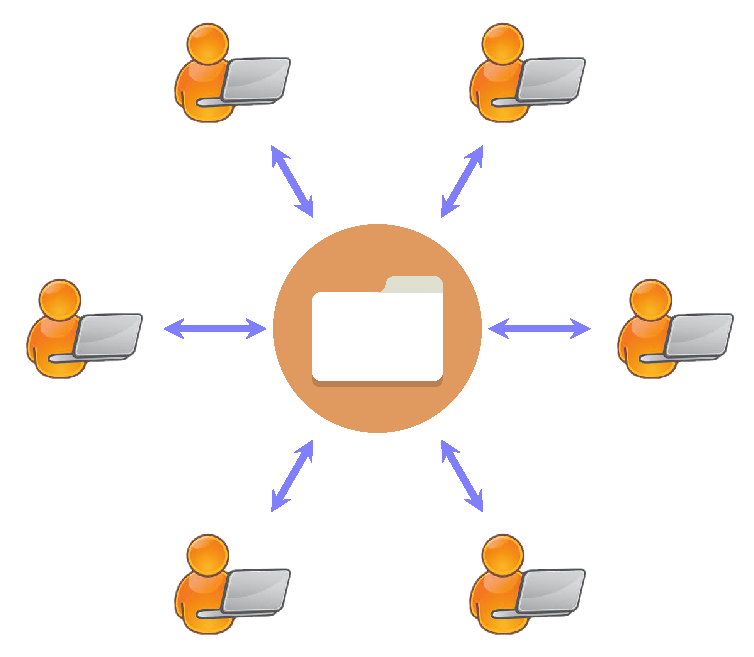
\includegraphics[height = 3cm]{shared-data-clients.pdf}};
  \node (dist) [right = 8.0cm of share] {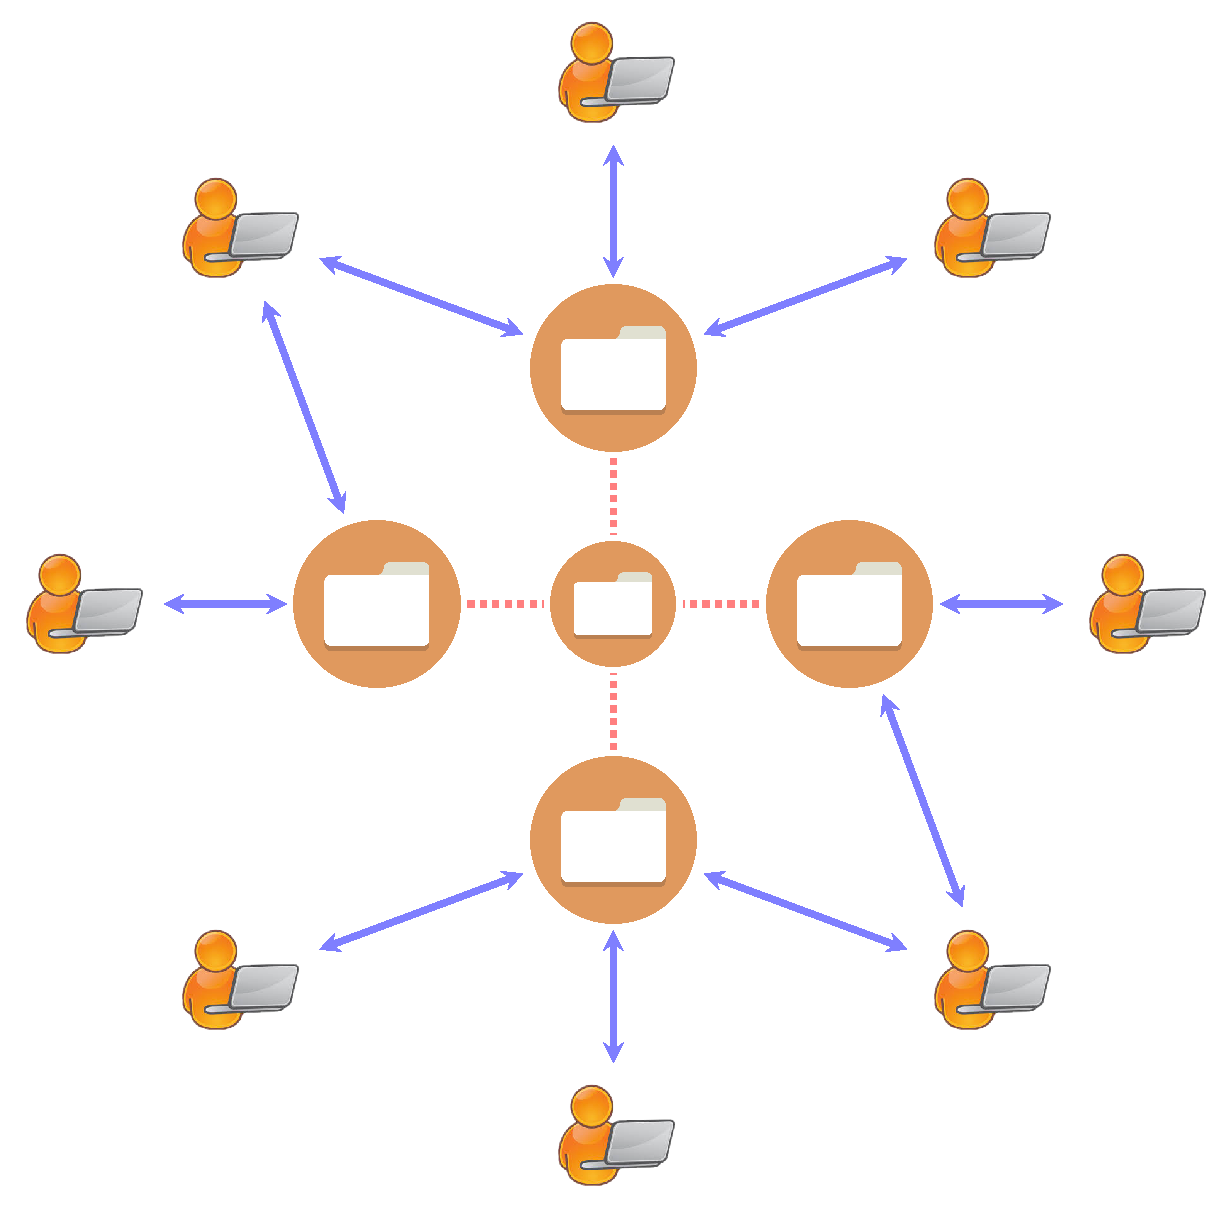
\includegraphics[height = 3.5cm]{distributed-data-clients.pdf}};

  % from (share) to (dist)
  \draw [-Implies, brown, line width = 1pt, double distance = 2pt, bend right = 35] (share) to node [black, sloped, below = 8pt] {{\bf Problem:} distributed data consistency problem.} (dist);

  % from (dist) to (share)
  \draw [-Implies, brown, line width = 1pt, double distance = 2pt, bend right = 35] (dist) to node () [black, sloped, above = 8pt] 
  {{\bf Idea:} distributed data behaves like shared data.} (share);

  % middleware
  \node (dsds) at ($(share.center)!0.5!(dist.center)$) {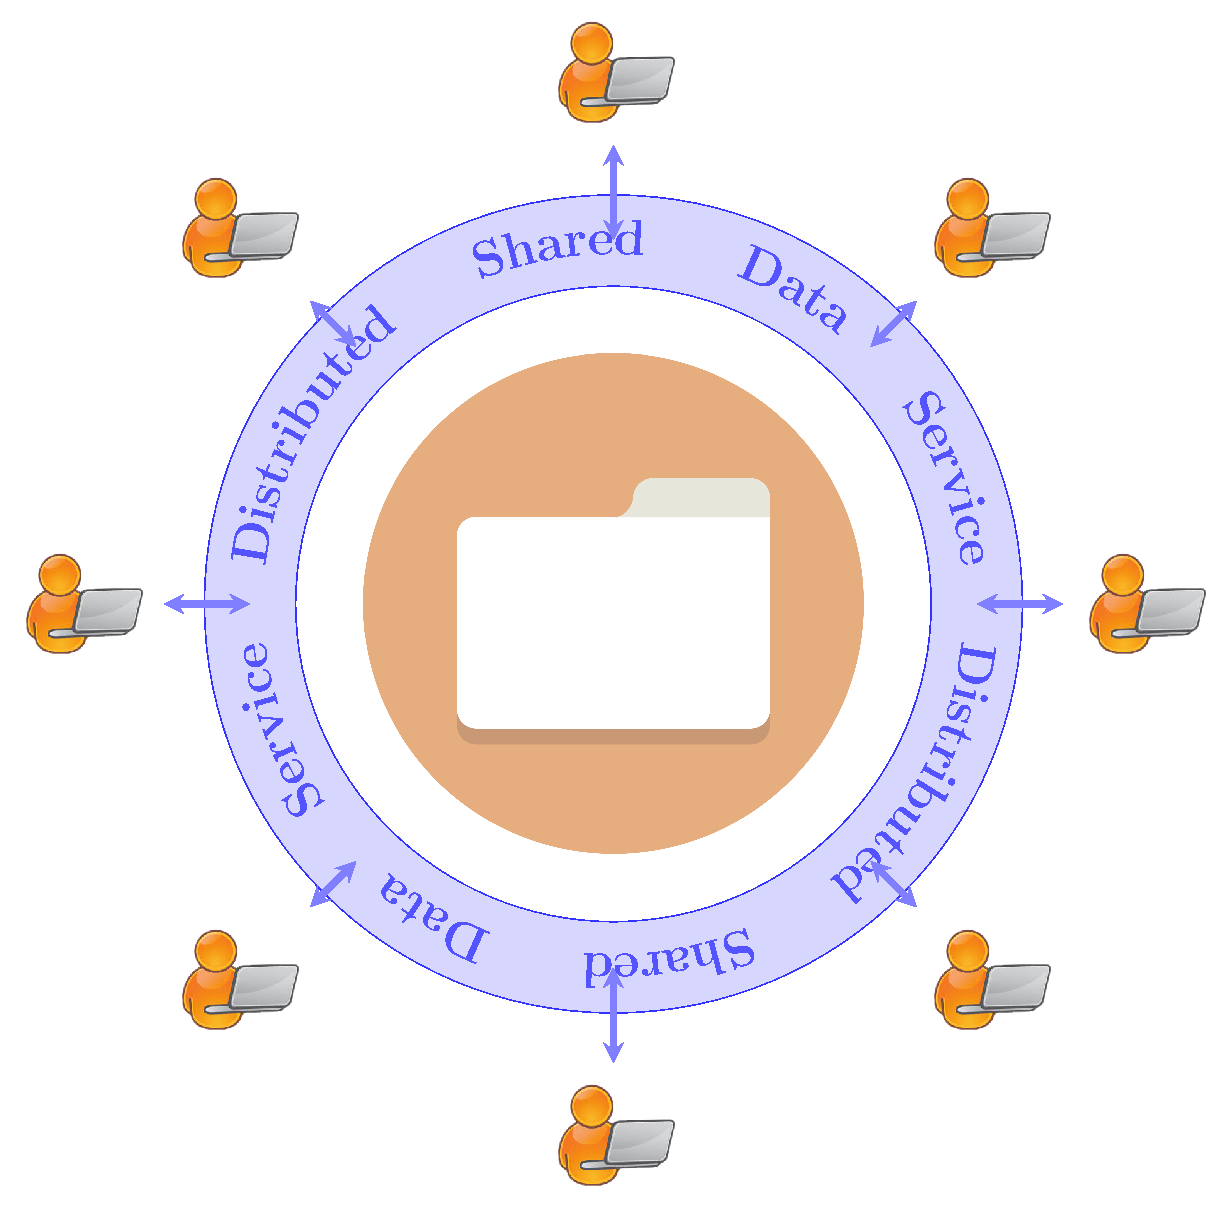
\includegraphics[height = 4.5cm]{distributed-shared-data-clients.pdf}};
  \draw [-Implies, blue!60, line width = 1pt, double distance = 1pt] (dist) to (dsds);
  \draw [-Implies, blue!60, line width = 1pt, double distance = 1pt] (dsds) to (share);
\end{tikzpicture}
\end{document}